\subsection*{الف}
در \lr{ZOH} با بزرگ‌نماییِ ضریب $2$، هر پیکسل به یک بلوک $2\times 2$ با همان مقدار تبدیل می‌شود؛ بنابراین یک مربعِ $4\times 4$ با مقدار $8$ در مرکزِ تصویر $8\times 8$ تشکیل می‌شود و بقیهٔ نواحی صفر می‌مانند (ظاهر کاملاً پله‌ای و \lr{blocky}).

\begin{center}
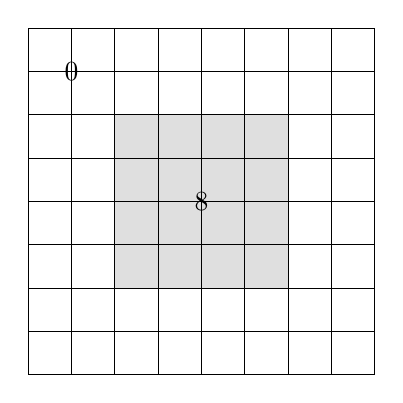
\begin{tikzpicture}[scale=0.55]
    % central 4x4 block (value 8)
    \fill[gray!25] (2,2) rectangle (6,6);

    % 8x8 grid
    \draw (0,0) grid (8,8);

    % minimal labels
    \node at (4,4) {$8$};
    \node at (1,7) {$0$};
\end{tikzpicture}
\end{center}

\subsection*{ب}
در بزرگ‌نمایی با ضریب $2$ به روش \lr{FOH} (در ۲بعد عملاً \lr{bilinear interpolation})، مقادیر بین نمونه‌ها به‌صورت خطی تغییر می‌کنند. بنابراین:
\begin{itemize}
    \item داخل ناحیهٔ مرکزی (بین پیکسل‌های ۸ مجاور) یک \lr{plateau} با مقدار نزدیک به $8$ باقی می‌ماند.
    \item در مرز بین $0$ و $8$ یک ناحیهٔ گذارِ نرم ایجاد می‌شود (مثلاً نمونهٔ میانی بین $0$ و $8$ مقدار $4$ می‌گیرد).
    \item گوشه‌های مرز (جایی که یک $8$ با چند $0$ همسایه است) مقادیر کوچک‌ترِ میانی تولید می‌کنند (مثل $2$ در مرکزِ یک سلول که سه گوشه‌اش صفر و یکی‌اش ۸ است).
\end{itemize}
پس ظاهر کلی: یک مربع روشن در مرکز که لبه‌های آن به‌جای پله‌ای، به‌صورت رمپ‌های خطی/محو شونده به زمینهٔ صفر وصل می‌شود.

\subsection*{ج}
\lr{cubic spline interpolation} معمولاً طبیعی‌تر از \lr{ZOH} و \lr{FOH} است چون:
\begin{itemize}
    \item پیوستگی مرتبهٔ بالاتری دارد (معمولاً پیوستگی تا مشتق دوم)، پس لبه‌ها و تغییرات شدت نرم‌تر و چشم‌پسندتر می‌شوند.
    \item نسبت به \lr{ZOH} (بلوک‌بلوک شدن) و \lr{FOH} (شکستگی در مشتق/ظاهر \lr{piecewise-linear}) مصنوعات دیداری کمتری ایجاد می‌کند.
    \item تقریب بهتری از یک بازسازی پایین‌گذر (ایدهٔ بازسازی سیگنال هموار) ارائه می‌دهد، لذا نتیجه کمتر مصنوعی دیده می‌شود.
\end{itemize}

\subsection*{د}
اگر هر حسگر به‌جای نمونه‌برداری نقطه‌ای، روی یک مربع کوچک میانگین‌گیری کند، اثر \lr{finite aperture} داریم.

\begin{itemize}
    \item در حوزهٔ مکانی: تصویر ایده‌آل با تابع پخش نقطه‌ایِ مربعی هم‌پیچیده می‌شود؛ یعنی یک \lr{blur} از نوع میانگین‌گیر (جعبه‌ای) رخ می‌دهد.
    \[
    g(x,y) = f(x,y) * h(x,y), \qquad
    h(x,y)=\frac{1}{A}\,\Pi\!\left(\frac{x}{a}\right)\Pi\!\left(\frac{y}{a}\right)
    \]
    \item در حوزهٔ فرکانس: طیف تصویر در پاسخ فرکانسی دریچه ضرب می‌شود و مؤلفه‌های فرکانس بالا تضعیف می‌گردند:
    \[
    G(u,v)=F(u,v)\,H(u,v),\qquad
    H(u,v)\propto \mathrm{sinc}(au)\,\mathrm{sinc}(av).
    \]
\end{itemize}

\subsection*{هـ}
همین اثر می‌تواند هم مضر و هم مفید باشد:
\begin{itemize}
    \item مضر: تضعیف فرکانس‌های بالا باعث کاهش وضوح، محوشدن لبه‌ها و از دست رفتن جزئیات ریز می‌شود.
    \item مفید: چون یک پایین‌گذرِ فیزیکی ایجاد می‌کند، می‌تواند آلیاسینگ را کاهش دهد (نقش \lr{anti-aliasing} قبل از نمونه‌برداری) و همچنین بخشی از نویزِ فرکانس‌بالا را کم کند.
\end{itemize}

\subsection*{و}
اگر طیف تصویر تقریباً دایره‌ای باشد، از دید هندسی نمونه‌برداری شش‌ضلعی کاراتر است چون:
\begin{itemize}
    \item در حوزهٔ فرکانس، ناحیهٔ نایکوئیستِ شبکهٔ نمونه‌برداری همان سلول بنیادیِ شبکهٔ دوگان است؛ برای شبکهٔ شش‌ضلعی این ناحیه یک شش‌ضلعی منتظم است که نسبت به مربع، به دایره نزدیک‌تر است.
    \item چون پشتیبانی طیف دایره‌ای است، قرار دادنِ دایره داخل شش‌ضلعی «هدررفت فضا»ی کمتری نسبت به قرار دادن داخل مربع دارد؛ پس برای پوشش یک طیف دایره‌ای با همان حاشیهٔ عدم‌همپوشانی، می‌توان با چگالی نمونه‌برداری کمتر (یا با همان چگالی، باند عبور بزرگ‌تر) کار کرد.
\end{itemize}